\documentclass[4pt,usenames,dvipsnames,aspectratio=169,table]{beamer}
%\usetheme{cern}
\usetheme{cernomc}

% Beamer Setup ---
\setbeamercovered{transparent=5} 
\setbeamertemplate{navigation symbols}{} 

\AtBeginSection{%
	\begin{frame}[noframenumbering]{Outline}
	\tableofcontents[currentsection]
	\end{frame}
}

% Imports ---
\usepackage[utf8]{inputenc}
\usepackage{amsmath}
\usepackage{amsfonts}
\usepackage{amssymb}
\usepackage{unicode-math}
\usepackage{mathtools}
\usepackage{bm}  % bold math
\usepackage{graphicx}
\usepackage{grffile}  % filenames with dots 
\usepackage{fontawesome5}

\usepackage{tikz}
\usetikzlibrary{calc}

\usepackage{hyperref}
\usepackage{siunitx}
\usepackage{booktabs}
\usepackage{multirow}
\usepackage{caption}
\usepackage[absolute,overlay]{textpos}

\usepackage{fontspec}
\usefonttheme{serif}
%\setmainfont{STIX Two Text}
%\setmathfont{STIX Two Math}
\setmainfont{TeX Gyre Bonum}
\setmathfont{TeX Gyre Bonum Math}


% some shenanigans -------------------------------------------------------------
\newcommand{\highl}[1]{\textbf{#1}}
\definecolor{RunTwored}{RGB}{200,0,0}
\definecolor{APJgreen}{RGB}{20,150,0}
\definecolor{SbSorange}{RGB}{240,150,0}
\newcommand{\we}{\cellcolor{blue!20!white}}
\newcommand{\ho}{\cellcolor{red!20!white}}
\newcommand{\wh}{\cellcolor{green!20!white}}
\newcommand{\bonelabel}{%
        \node at ($(b1) +(-0.13\linewidth, 0.15\linewidth)$) {\sffamily\small\textbf{Beam 1}};
}
\newcommand{\btwolabel}{%
        \node at ($(b2) +(-0.13\linewidth, 0.15\linewidth)$) {\sffamily\small\textbf{Beam 2}};
}

% highly illegal!
\newcommand{\faSunrise}{
\includegraphics[width=1.2em]{sunrise.png}}


% Meta -------------------------------------------------------------------------
\author[OMC]{%
Andreas Wegscheider on behalf of the OMC team:\\%
\small
T.~Persson,  F.~Carlier, A.~Costa~Ojeda, J.~Dilly, H. Garc\'ia Morales, V.~Ferrentino, 
 E.~Fol, M.~Hofer, E.J~Høydalsvik, J.~Keintzel, M.~Le~Garrec, E.H.~Maclean,    
 L.~Malina, F.~Soubelet, R.~Tom\'as, L.~Van Riesen-Haupt and A.~Wegscheider, CERN, Geneva, Switzerland \\
  J. Cardona, Universidad Nacional de Colombia\\[1em]
% hacky, I know ...
\centering%

\includegraphics[width=3cm]{OMC_logo_original.pdf}%
\\
\textbf{Thanks to}
J\"org Wenninger, Matteo Solfaroli Camillocci, the coordinators and EICs who helped with the measurements,
Stephane Fartoukh, Riccardo de Maria and Michi Hostettler
}
\title[LHC 2022]{LHC Commissioning 2022}
\logo{} 
\titlegraphic{}
\institute{CERN}
\date[09.06.22]{09.06.2022}
\subject{} 

% Document ---------------------------------------------------------------------
\begin{document}

\begin{frame}
    \titlepage
\end{frame}


\begin{frame}{Full Outline}
\tableofcontents
\end{frame}

\section{OMC Procedures and Shifts}

\begin{frame}{Shift Schedule }

    %\textbf{note:} this is just to collect now, will be cleaned for presentation

    \begin{minipage}{0.40\linewidth}
    \footnotesize
    \begin{tabular}{ll|ll|ll}
        \multicolumn{2}{c}{April}
        &\multicolumn{2}{c}{May}
        &\multicolumn{2}{c}{June}\\
    %date & actual            & date & actual          & date & actual            \\
    \wh 22. & \wh \faSun           &     02.   &           \faMoon   & \we 03.   & \we       \faMoon    \\
    \we 23. & \we\faSun            &     05.   &    \faMoon          & \we 04.   & \we       \faMoon    \\
    \we 24. & \we\faSun\faMoon     & \we 07.   & \we\faMoon          & \ho 06.   & \ho\faSun            \\
    \wh 25. & \wh\faSun            & \we 08.   & \we\faSunrise\faMoon& \wh 09.   & \wh\faSun \faMoon    \\
        27. &    \faMoon           &     09.   &    \faSunrise\faMoon&           &                      \\
        28. &    \faSunrise\faMoon & \we 20.   & \we\faMoon          &           &                      \\
            &                      & \ho 26.   & \ho\faMoon          &           &                      \\
            &                      & \ho 27.   & \ho\faMoon          &           &                      \\
            &                      & \ho 28.   & \ho\faMoon          &           &                      \\
            &                      & \ho 29.   & \ho\faSun \faMoon   &           &                      \\
            &                      & \ho 31.   & \ho\faMoon          &           &                      \\
        \hline
    %    \multicolumn{2}{c|}{2(3)\faMoon / 6 }
    %    &\multicolumn{2}{c|}{5(7)\faMoon / 11}
    %    &\multicolumn{2}{c}{0(2)\faMoon / 3}
    \end{tabular}\\
    \footnotesize

    \begin{tabular}{lll}
    \faSunrise: morning& \faSun: day& \faMoon: night\\
    \we weekend  & \ho holiday &\wh working hours
    \end{tabular}
    \end{minipage}
    \begin{minipage}{0.59\linewidth}
    \normalsize

    \footnotesize
    \begin{itemize}
        \item out of 21 shifts, many on holidays / weekends (\highl{11}), \highl{only 3} during working hours
        \item people who are \highl{not full-time} LHC\\
        {\footnotesize(FCC, myon colliders, injectors)}
        \item more than 3 years of Run~2 commissioning condensed into a \highl{few months}
        \item \highl{4 optics} (Nominal, Ballistic, Van-der-Meer, 60 degrees)
        \only<1>{\item much work outside working hours, team of dedicated night owls}
        \begin{center}
            \only<2>{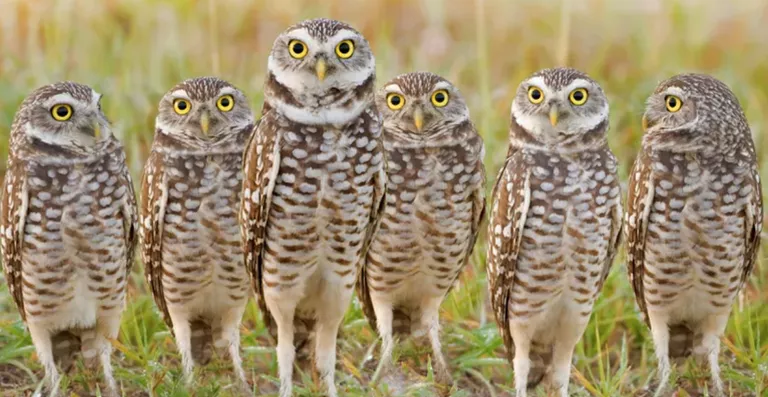
\includegraphics[width=0.8\linewidth]{images/owls/omc_team1.png}}
        \end{center}
    \end{itemize}
    \normalsize

    \end{minipage}

\end{frame}

\begin{frame}
    \frametitle{Optics Measurements}

    \begin{minipage}{0.55\linewidth}
    \begin{center}
        \begin{tikzpicture}
            \node (b1) {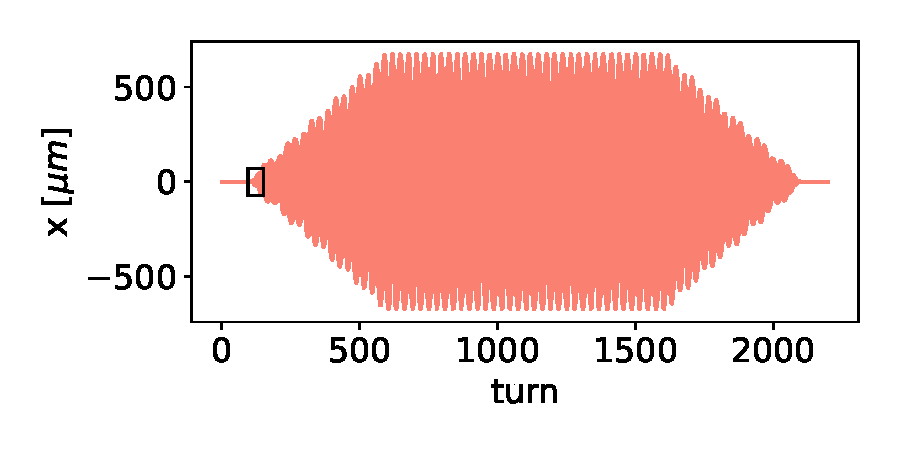
\includegraphics[width=.8\linewidth]{images/acdipole/ac_plot}};
            \node at ($(b1) + (1.1,1.1)$) {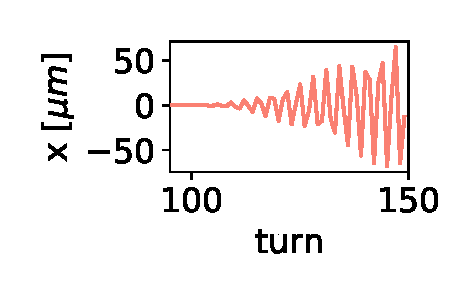
\includegraphics[width=.35\linewidth]{images/acdipole/ac_plot_zoom}};
        \end{tikzpicture}
    \end{center}

            \footnotesize
        \begin{itemize}
        \item use AC-dipole excitation to get turn-by-turn data
        \item adiabatic ramp up, no emittance blow-up
        \item has to be compensated
        \item high amplitude limited by machine protection
        \end{itemize} 
        \normalsize
    \end{minipage}
    %
    \begin{minipage}{0.44\linewidth}
        \textbf{Model dependent analysis}\\[-0.5em]
        \footnotesize
        \begin{itemize}
            \item many of our algorithms depend on model values
            \item need good knowledge of machine configuration
        \end{itemize}
        
        \textbf{Some references}
        
        \tiny
        T.~Persson et al,
        \emph{Improved control of the betatron coupling in the Large Hadron Collider},
        \href{https://cds.cern.ch/record/2135848?ln=en}{\faExternalLink*}
        \\[-0.5em]
        
        T.~Persson et al,
        \emph{LHC optics commissioning: A journey towards 1\% optics control},
        \href{https://journals.aps.org/prab/abstract/10.1103/PhysRevAccelBeams.20.061002}{\faExternalLink*}
        \\[-0.5em]
        
        A.~Wegscheider et al,
        \emph{Analytical N beam position monitor method},
        \href{https://journals.aps.org/prab/abstract/10.1103/PhysRevAccelBeams.20.111002}{\faExternalLink*}
        \\[-0.5em]
        
        \emph{Chapter about Physics on the OMC website}
        \href{https://pylhc.github.io/measurements/physics}{\faExternalLink*}
        
        \normalsize
        
    \end{minipage}
\end{frame}


\begin{frame}{Dedicated Collimation Sequence}

    \begin{itemize}
        \item \highl{dedicated} collimation sequence to be trimmed in for \highl{OMC measurements}
        \item two settings: \highl{injection} and \highl{top energy}
        \item \highl{automates} collimation setup
        \item crucial to get sufficient \highl{kick amplitude} at top energy
        \item benefitial for linear and non-linear measurements
        \item no need to call collimation expert during night shift on a holiday
        \item \highl{huge effort} from collimation, whole shift to measure and prepare the sequence
    \end{itemize}

\end{frame}


\section{Model Creation}


\begin{frame}{Model Creation}

\begin{itemize}
    \item having an \emph{online model} that represents the current lattice configuration is a \highl{challenging task}
    \item several attempts in the past
    \item OMC-OP workshop: decision to create \highl{central optics repository}
    \item  global effort \highl{OP}+\highl{ABP}, combining \highl{\href{https://gitlab.cern.ch/acc-models}{acc-models \faExternalLink*}} (repository of design optics) with
LSA (online information about trimmed-in knobs, \highl{StateTracker})
    %\item (TODO: insert sketch of workflow)
    %\item still not fully adapted: up to June 2nd trim to wrong place
    %("We all need to get used to this, people are still used to trim everything on correction..." -- Michi)
    \item \highl{huge effort} from OP to change usage {\footnotesize(trim on target instead of correction)}
    \item still ongoing effort from both OP and ABP
\end{itemize}

\end{frame}


\section{Linear Optics}


\begin{frame}{30\,cm Optics -- record high $\beta$~beating}

    \begin{tikzpicture}
        \node[above left] (b1) {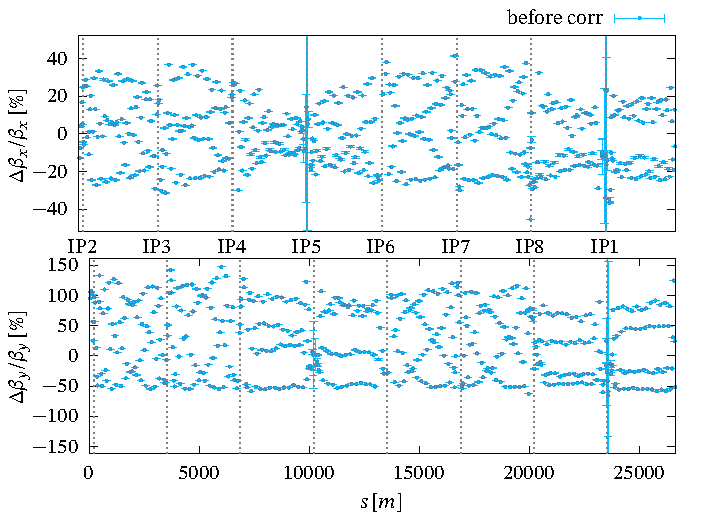
\includegraphics[width=0.5\linewidth]{images/squeeze/b1_recordhigh.pdf}};
        \bonelabel
        \node (b2) at ($(b1) + (0.5\linewidth,0)$)
            {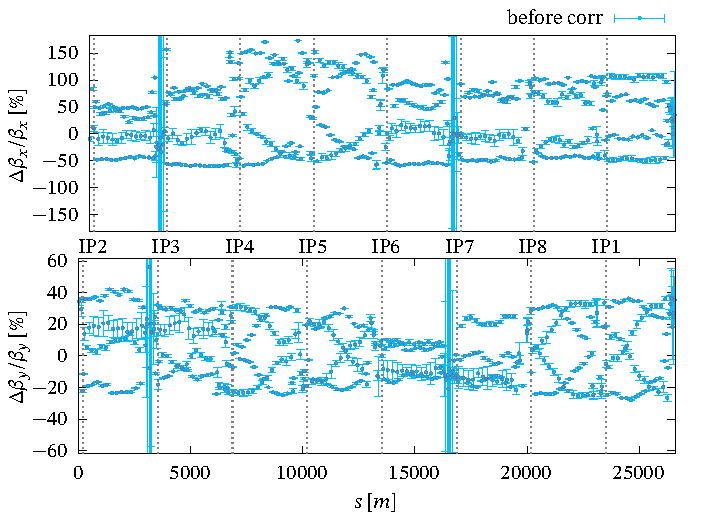
\includegraphics[width=0.5\linewidth]{images/squeeze/b2_recordhigh.pdf}};
        \btwolabel
    \end{tikzpicture}
    
    \begin{itemize}
        \item peak $\beta$~beating of \textbf{150 \%}
        \item highest ever measured in the LHC
        \item first time ATS factor 2 (before it was 1.33 at \SI{30}{cm})
    \end{itemize}
    
\end{frame}


\begin{frame}{30\,cm Optics}
    \begin{center}
        \only<2>{
            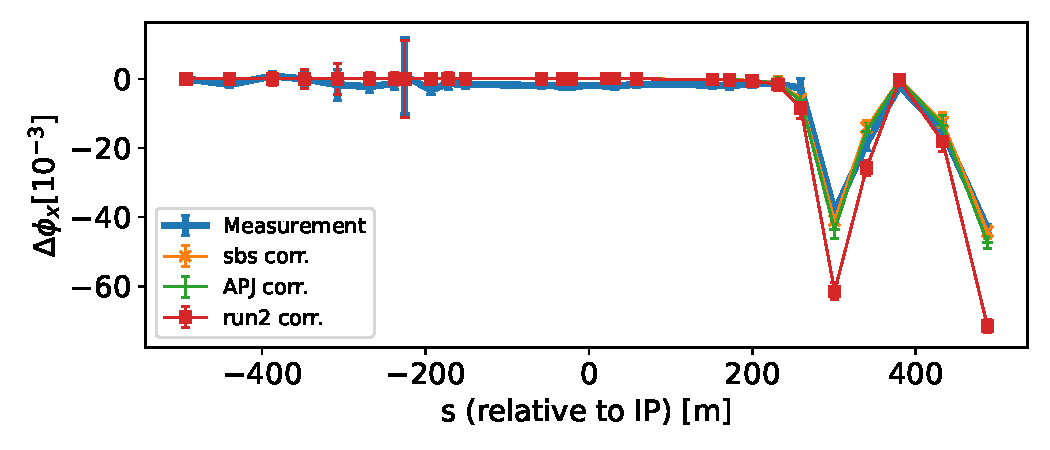
\includegraphics[width=0.8\linewidth]{images/flattop/beam2_x_IP1.pdf}
        }
        \only<1>{
        {\tiny
         \begin{tabular}{l|lSSSS|c|} \toprule
              & \textbf{Circuit}%
              & \multicolumn{4}{c|}{$\Delta k (10^{-5}\SI{}{m^{-2}})$}
              & \textbf{Polarity}%
              \\ \cmidrule{2-6}
              &
              & \multicolumn{1}{c}{\color{RunTwored}\textbf{Run 2}}
              &{\color{APJgreen}\textbf{APJ}}
              &{\color{SbSorange}\textbf{SbS}}
              &{\textbf{ML}}
              & \textbf{LSA} \\\hline \midrule
     IR1 & \texttt{ktqx1.l1} & \color{RunTwored} 1.23 & \color{APJgreen} 0    & \color{SbSorange} 1.23 &  1.23 & - \\
         & \texttt{ktqx1.r1} & \color{RunTwored}-1.23 & \color{APJgreen} 0    & \color{SbSorange}-1.23 & -1.24 & + \\
         & \texttt{ktqx2.l1} & \color{RunTwored} 0.65 & \color{APJgreen} 1.15 & \color{SbSorange} 0.41 & -0.11 & + \\
         & \texttt{ktqx2.r1} & \color{RunTwored}-1.0  & \color{APJgreen}-0.87 & \color{SbSorange}-0.70 &  0.18 & - \\
         & \texttt{ktqx3.l1} & \color{RunTwored} 1.22 & \color{APJgreen} 1.94 & \color{SbSorange} 1.22 &  0.31 & - \\
         & \texttt{ktqx3.r1} & \color{RunTwored}-1.22 & \color{APJgreen}-2.88 & \color{SbSorange}-1.22 & -0.1  & + \\\hline \midrule
     IR5 & \texttt{ktqx1.l5} & \color{RunTwored} 2.0  & \color{APJgreen} 0    & \color{SbSorange} 2.25 & \text{-} & - \\
         & \texttt{ktqx1.r5} & \color{RunTwored}-2.0  & \color{APJgreen} 0    & \color{SbSorange}-2.10 & \text{-} & + \\
         & \texttt{ktqx2.l5} & \color{RunTwored} 0.26 & \color{APJgreen} 0.38 & \color{SbSorange} 0.16 & \text{-} & + \\
         & \texttt{ktqx2.r5} & \color{RunTwored} 1.48 & \color{APJgreen} 0.93 & \color{SbSorange} 1.35 & \text{-} & - \\
         & \texttt{ktqx3.l5} & \color{RunTwored} 1.49 & \color{APJgreen} 3.40 & \color{SbSorange} 2.25 & \text{-} & - \\
         & \texttt{ktqx3.r5} & \color{RunTwored}-1.49 & \color{APJgreen}-2.46 & \color{SbSorange}-2.10 & \text{-} & + \\\hline \midrule
        \end{tabular} 
        }
        }
    \end{center}
    \only<1>{
    \begin{itemize}
        \item measurements at $\beta^*=\SI{30}{\centi\meter}$ performed
        \item corrections calculated using \highl{APJ}, \highl{SbS}, \highl{ML} and taken from \highl{run2}
        \item ML correction yield good results but are \highl{less local}
    \end{itemize}
    }
    \only<2>{
    \begin{itemize}
        \item APJ and SbS yield \highl{similar corrections},
            run2 corrections are over-correcting when applied now
    \end{itemize}
    }
\end{frame}


\begin{frame}{30\,cm Optics -- before and after local corrs}

    %\begin{center}
        \begin{tikzpicture}
            \node (b1) {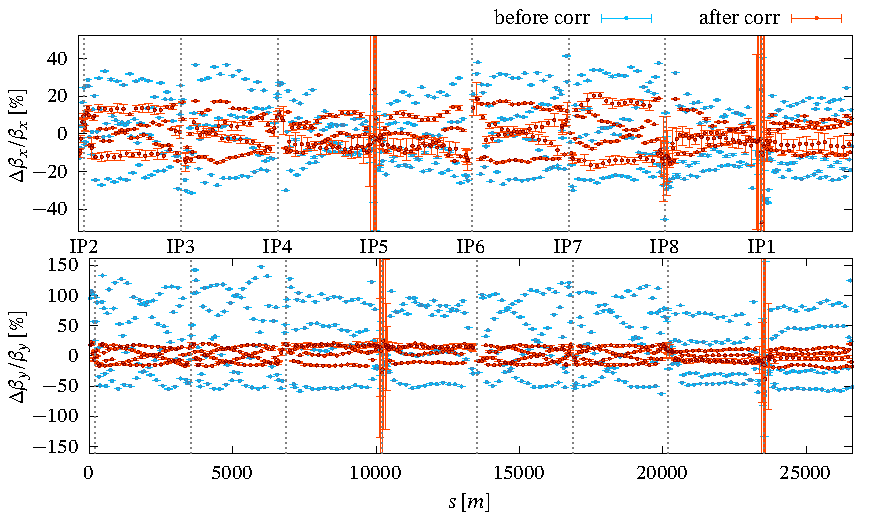
\includegraphics[width=0.52\linewidth]{images/squeeze/b1_bb_comp.pdf}};
            \node (b2) at ($(b1) + (0.52\linewidth,0)$) 
                {
\includegraphics[width=0.52\linewidth]{images/squeeze/b2_bb_comp.pdf}};
            \bonelabel   
            \btwolabel   
        \end{tikzpicture}
    %\end{center}
    \vspace{-0.5em}
    \small
    \begin{itemize}
        \item $\beta$~beating \highl{after implementation} of local corrections in IPs \textbf{1}, \textbf{2}, \textbf{5} and \textbf{8}
        \item IP1 correction is taken from \highl{APJ}, others from \highl{SbS}
        \item $\beta$~beating stays \highl{under 20\%}
    \end{itemize}
    \normalsize
    
\end{frame}


\begin{frame}{Arc45 and 81 correction bumps}

\begin{minipage}[b]{0.7\linewidth}
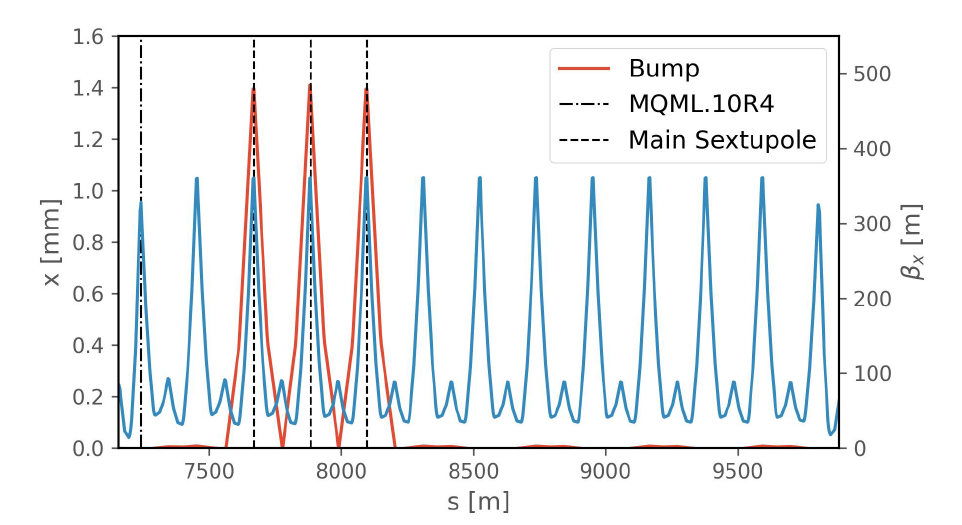
\includegraphics[width=\linewidth]{images/arcs/x_bumps.png}
\end{minipage}
\begin{minipage}[b]{0.29\linewidth}

\footnotesize
        \textbf{Orbit bump correction settings}
        
       \begin{tabular}{c|S}
       element & \text{correction}\\
       \hline
          \texttt{MCBH.16R4}  &  8e-6\\
          \texttt{MCBH.20R4}  &  16e-6\\
          \texttt{MCBH.24R4}  &  16e-6\\
          \texttt{MCBH.28R4}  &  8e-6\\
       \end{tabular}
       \vspace{0.5em}
       
        \textbf{Quad trim}
        
       \begin{tabular}{c|S}
       element & \text{correction}\\
       \hline
          \texttt{MQML.10R4}  &  2e-5\\
       \end{tabular}
       \vspace{1.5em}
       \normalsize
\end{minipage}

\begin{itemize}
    \item correction was found in Run~2 for flat optics using orbit bumps
    \item comparable phase deviation observed in Run~3
    \item correction bumps for Run~3 commissioning calculated
\end{itemize}
    
\end{frame}

\begin{frame}{Coupling Corrections}
    \begin{minipage}{0.55\linewidth}
        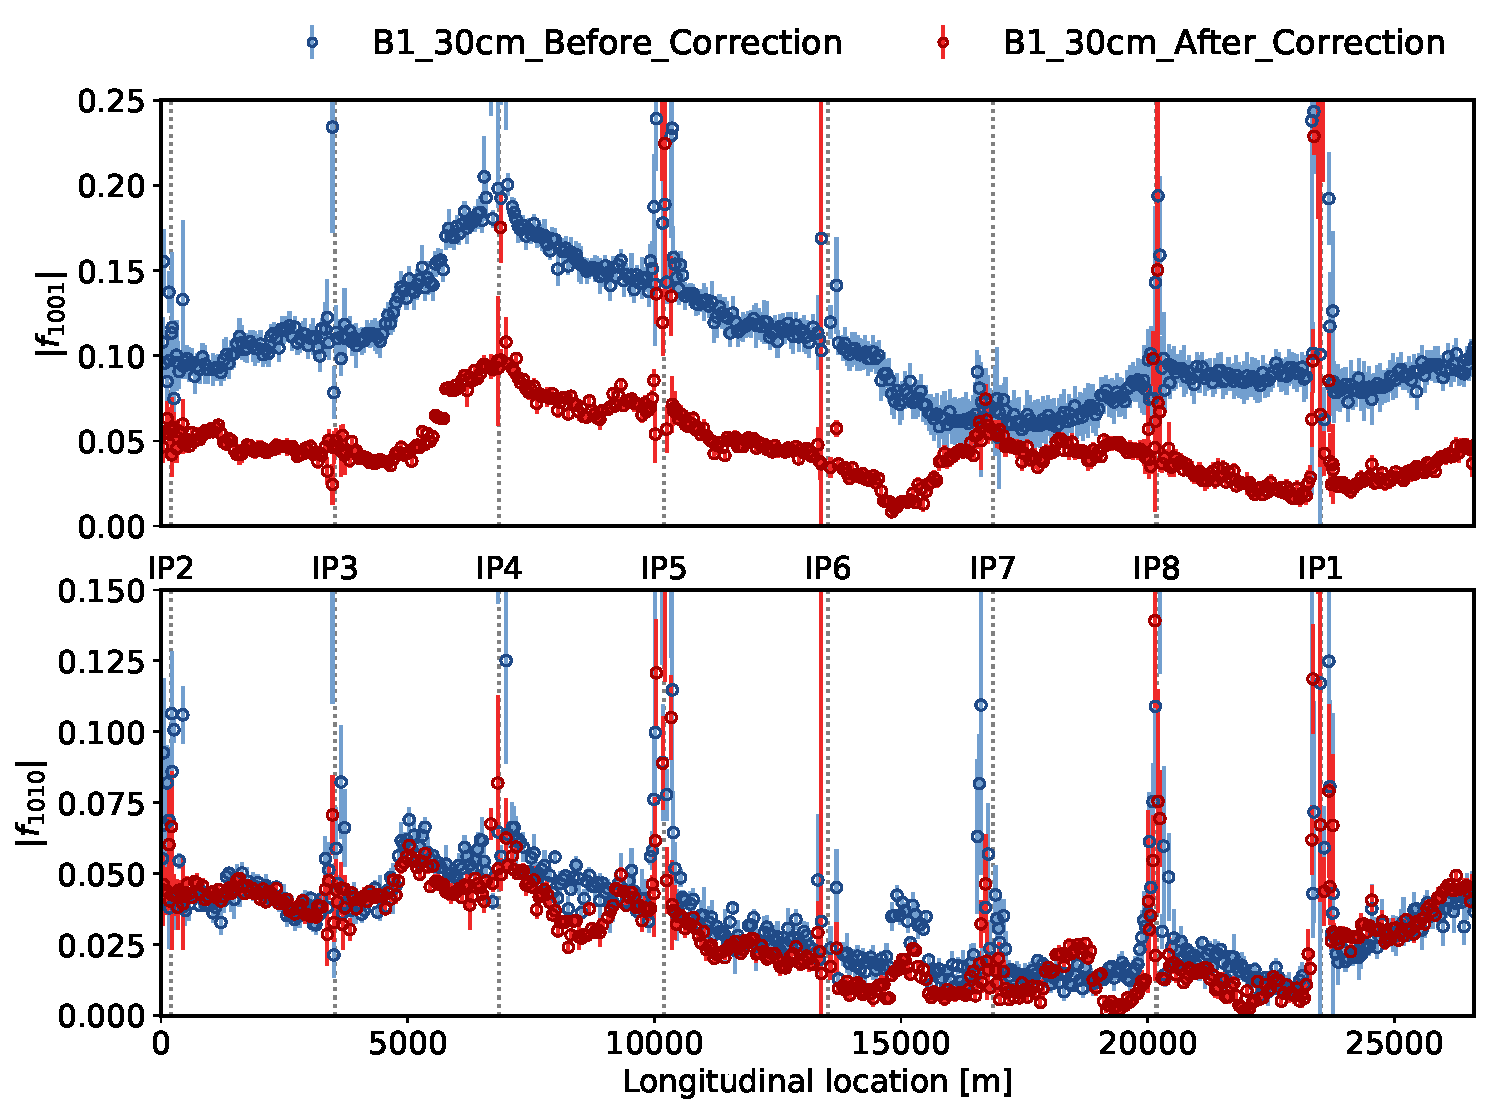
\includegraphics[width=\linewidth]{lhcb1_30cm_before_vs_after_arc_by_arc_coupling.pdf}
    \end{minipage}
    %
    \begin{minipage}{0.44\linewidth}
        \begin{itemize}
            \item local correction in the IPs
            \item B1 arc correction to flatten the coupling structure
            \item new method to find the right balance in the IPs (MQSX) between left and right,
            preliminary analysis indicates that it's close to optimal (IP1)
        \end{itemize}
    \end{minipage}
\end{frame}

%\begin{frame}{K Modulation after global corrections}
%\begin{center}
%   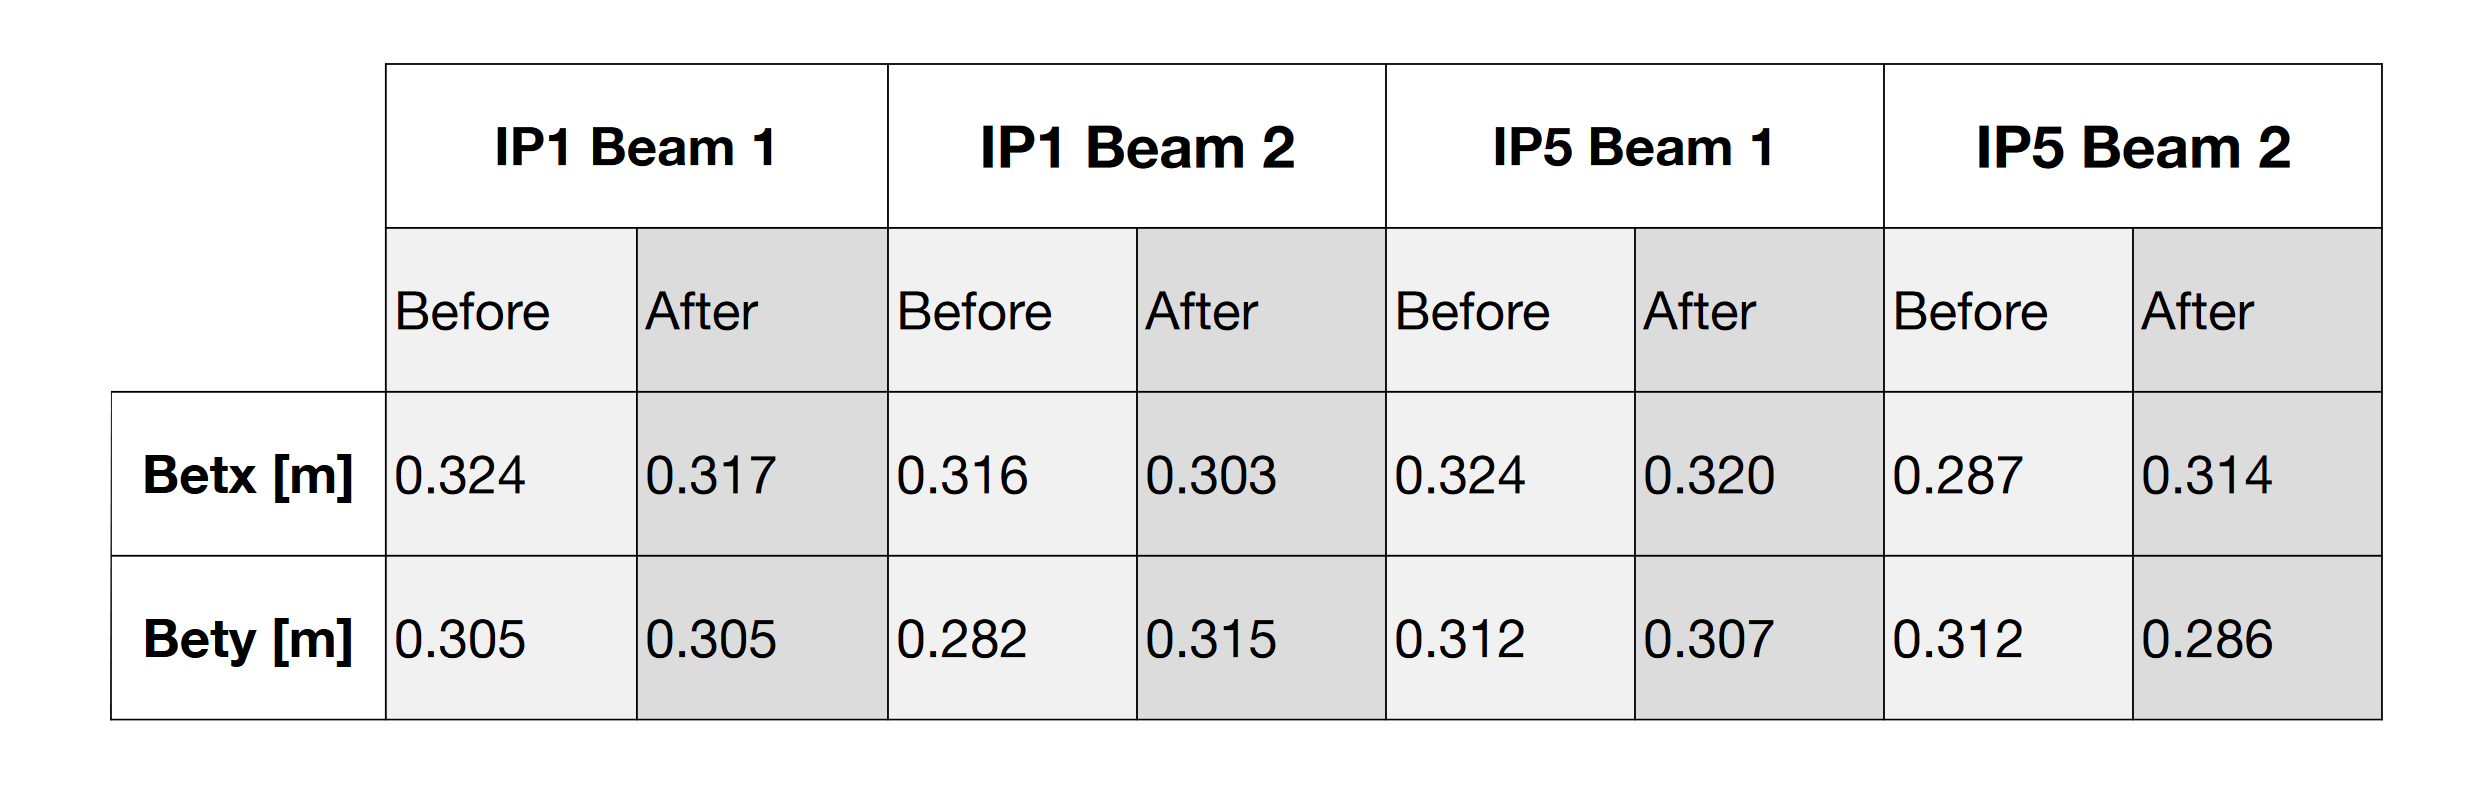
\includegraphics[width=0.7\linewidth]{kmod_after_global.png} 
%\end{center}
%\begin{itemize}
%    \item slight improvement
%    \item still $7\%$ $\beta$~beating at IP5 Beam 1
%\end{itemize}
%\end{frame}


%% Ballistic -------------------------------------------------------------------
%\section{Ballistic}
%\begin{frame}{Ballistic Optics}
%    
%\end{frame}
%
%
% Non-Linear ------------------------------------------------------------------
\section{Non-linear optics}

\begin{frame}{Amplitude Detuning at $\beta^*$ = 30cm, top energy}
    \begin{center}
        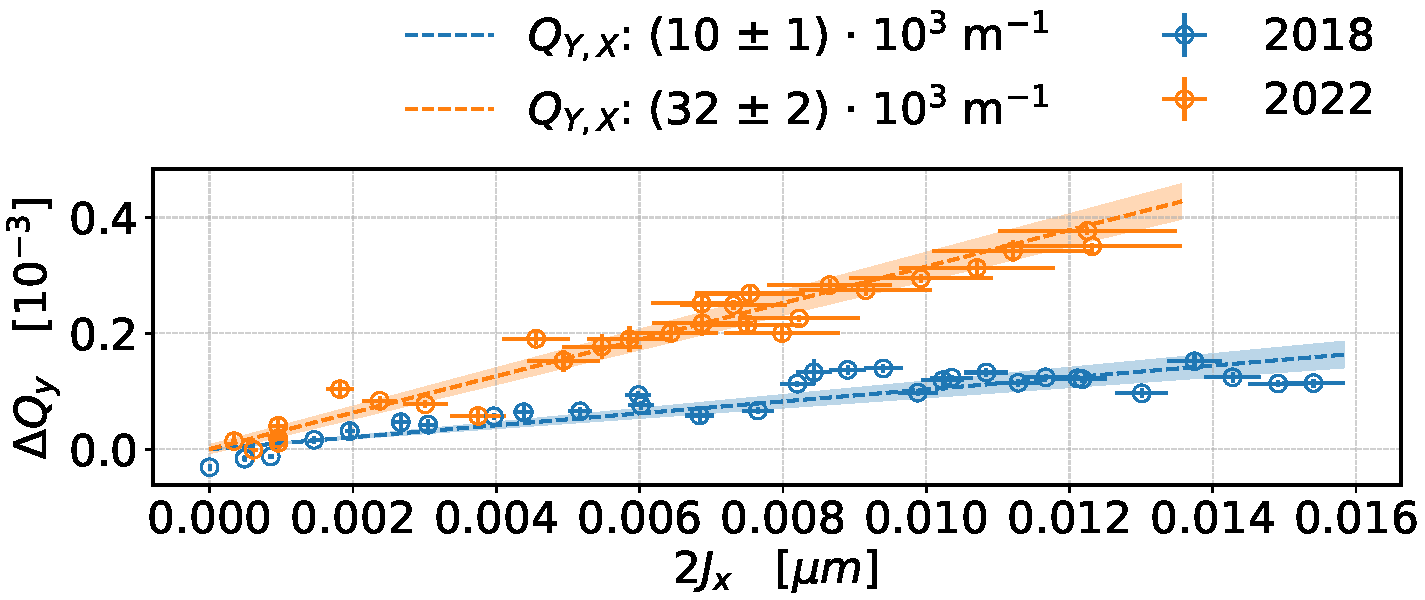
\includegraphics[width=0.5\linewidth]{images/nonlinear/comparison_2018_2022_dQYd2JX_corrected.pdf}
    \end{center}
    
    \small
    \begin{itemize}
        \item $Q''$, $Q'''$ and higher-order chroma at injection + corrections
        \item normal and skew sextupole corrections at end-of-squeeze
        \item \highl{first ever dodecapole} corrections in LHC
        \item cross term \highl{larger} than in run 2,
        with positive sign (should be negative for stability)
        \item at injection corrected to the level of \highl{previous years} with same corrections
    \end{itemize}
    \normalsize
\end{frame}


\section{Optics Reproducibility}

\begin{frame}{Reproducibility}


    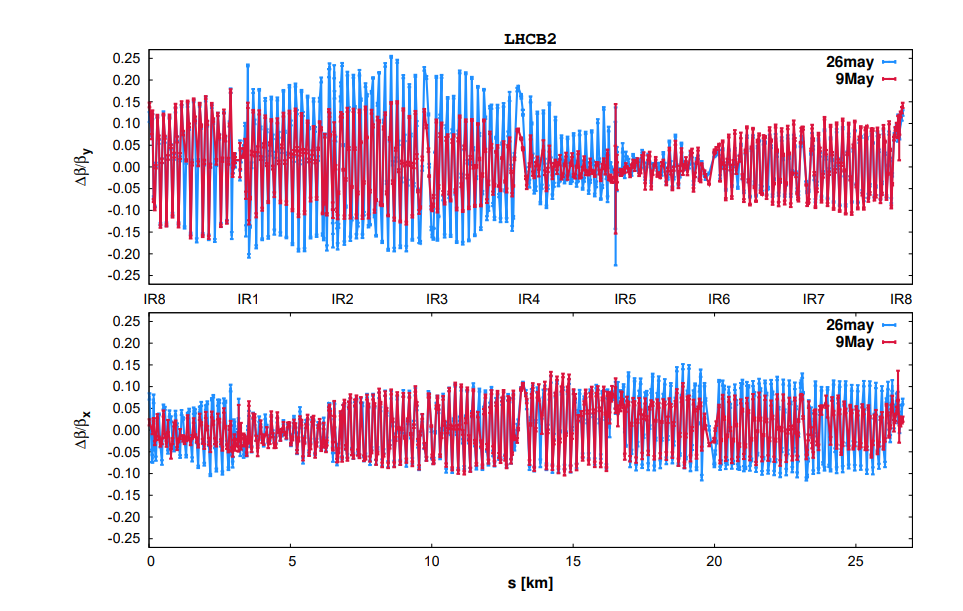
\includegraphics[width=0.5\linewidth]{images/reproducibility/B2_26May_9May.png}

\begin{itemize}
    \item \highl{big change} in $\beta$~beating between 9th May and 26th May (especially Beam 2)
    \item main hypothesis is the $dE/E$ shifts due to  \highl{orbit correction},
    to be confirmed by simulations / measurements
    \item  commissioning \highl{robust}, from 29 until today, reproducibility \highl{below 2 \%}
    %\item  full understanding \highl{ongoing}, will be covered later
\end{itemize}

    %for stephane: magnetic tcts ruled out 
    
\end{frame}

\section{Conclusion}

\begin{frame}
    \frametitle{Summary and Outlook}

    \begin{itemize}
        \item optics commissionning that has been spread out over all of run~2 is now done in one year
         \item \highl{many techniques}, e.g.: $Q''$ and $Q'''$ corrections, $b_4$,
        local corrections,
        feed-down from sextupoles in arcs, 
        $b_6$ corrections for the first time
        \item 4 different optics: \highl{Van-der-Meer, Ballistic, 60 degree, nominal}
        \item first time ATS factor 2 (before it was 1.33)
        \item are doing \highl{final steps} for commissioning now
        $\Rightarrow$ final configuration that we will \highl{leave in the machine}
        
        \item huge effort from participants, who often worked outside working hours but also from different sections, collimation and OP, that made this amount of commissioning possible
    \end{itemize}

\end{frame}


\begin{frame}{Publications from this commissioning}


        
        T.~Persson et al,
        \emph{
Optics correction strategy for Run 3 of the LHC	},
        \\[0.5em]
        
        
        J.F.~Cardona et al,
        \emph{PROGRESS ON ACTION PHASE JUMP FOR LHC LOCAL OPTICS
CORRECTION},
        \\[0.5em]
        

        E.~Fol et al,
        \emph{
Experimental Demonstration of Machine Learning Application in LHC Optics Commissioning
	},
        \\[0.5em]
    
\end{frame}


% --------------------------------------------------------------------------------------------------
% --- BACKUP ---------------------------------------------------------------------------------------
% --------------------------------------------------------------------------------------------------

\begin{frame}{}

\begin{center}
{\Huge \textbf{Backup Slides}}
\end{center}
    
\end{frame}


% Injection --------------------------------------------------------------------


\begin{frame}{Injection optics}
    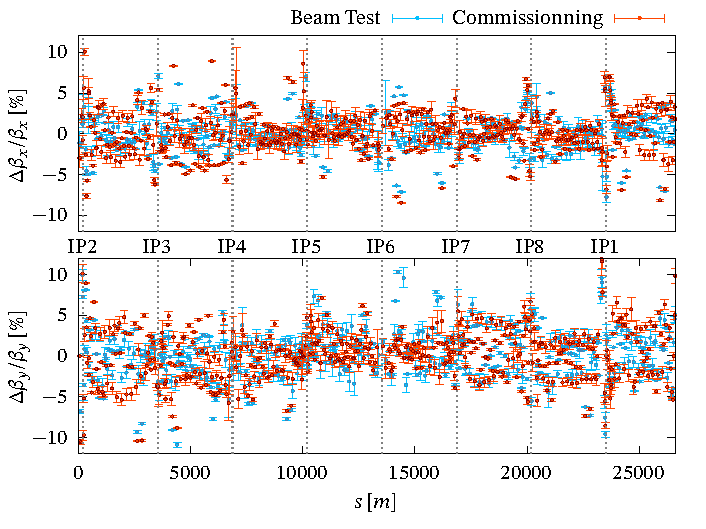
\includegraphics[width=0.49\linewidth]{images/beamtest/b1_bb.pdf}
    \hfill
    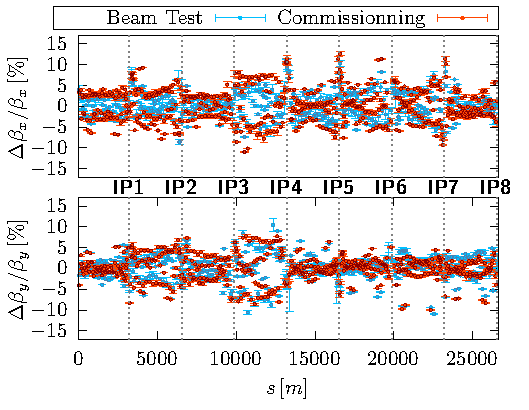
\includegraphics[width=0.49\linewidth]{images/beamtest/b2_bb.pdf}
    
    \begin{itemize}
        \item  Measured the injection optics with the corrections of \highl{2021 beam test}.
        \item Looks similar, \highl{no corrections} were re-calculated.
    \end{itemize}
\end{frame}


% Ramp -------------------------------------------------------------------------
% Flattop ---------------------------------------------------------------------


\begin{frame}{Flattop, $\beta$=133\,cm}
    
    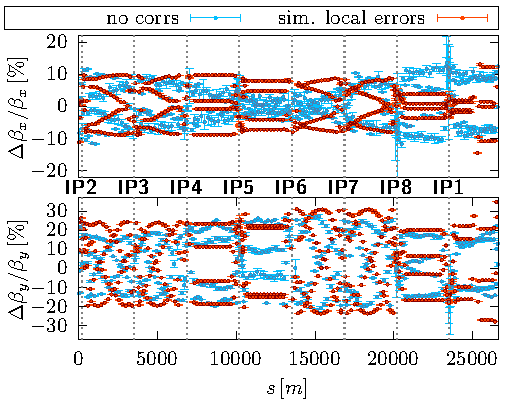
\includegraphics[width=0.49\linewidth]{images/flattop/b1_bb.pdf}
    \hfill
    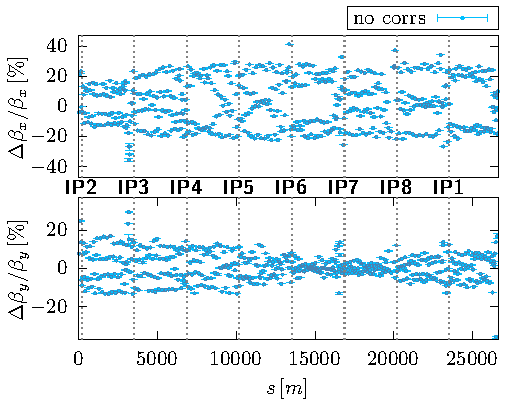
\includegraphics[width=0.49\linewidth]{images/flattop/b2_bb.pdf}
    \begin{itemize}
        \item measurements at \SI{6.8}{TeV} performed
        \item errors within tolerances, no dedicated corrections
    \end{itemize}
    
\end{frame}


\begin{frame}{Coupling in the Ramp}
    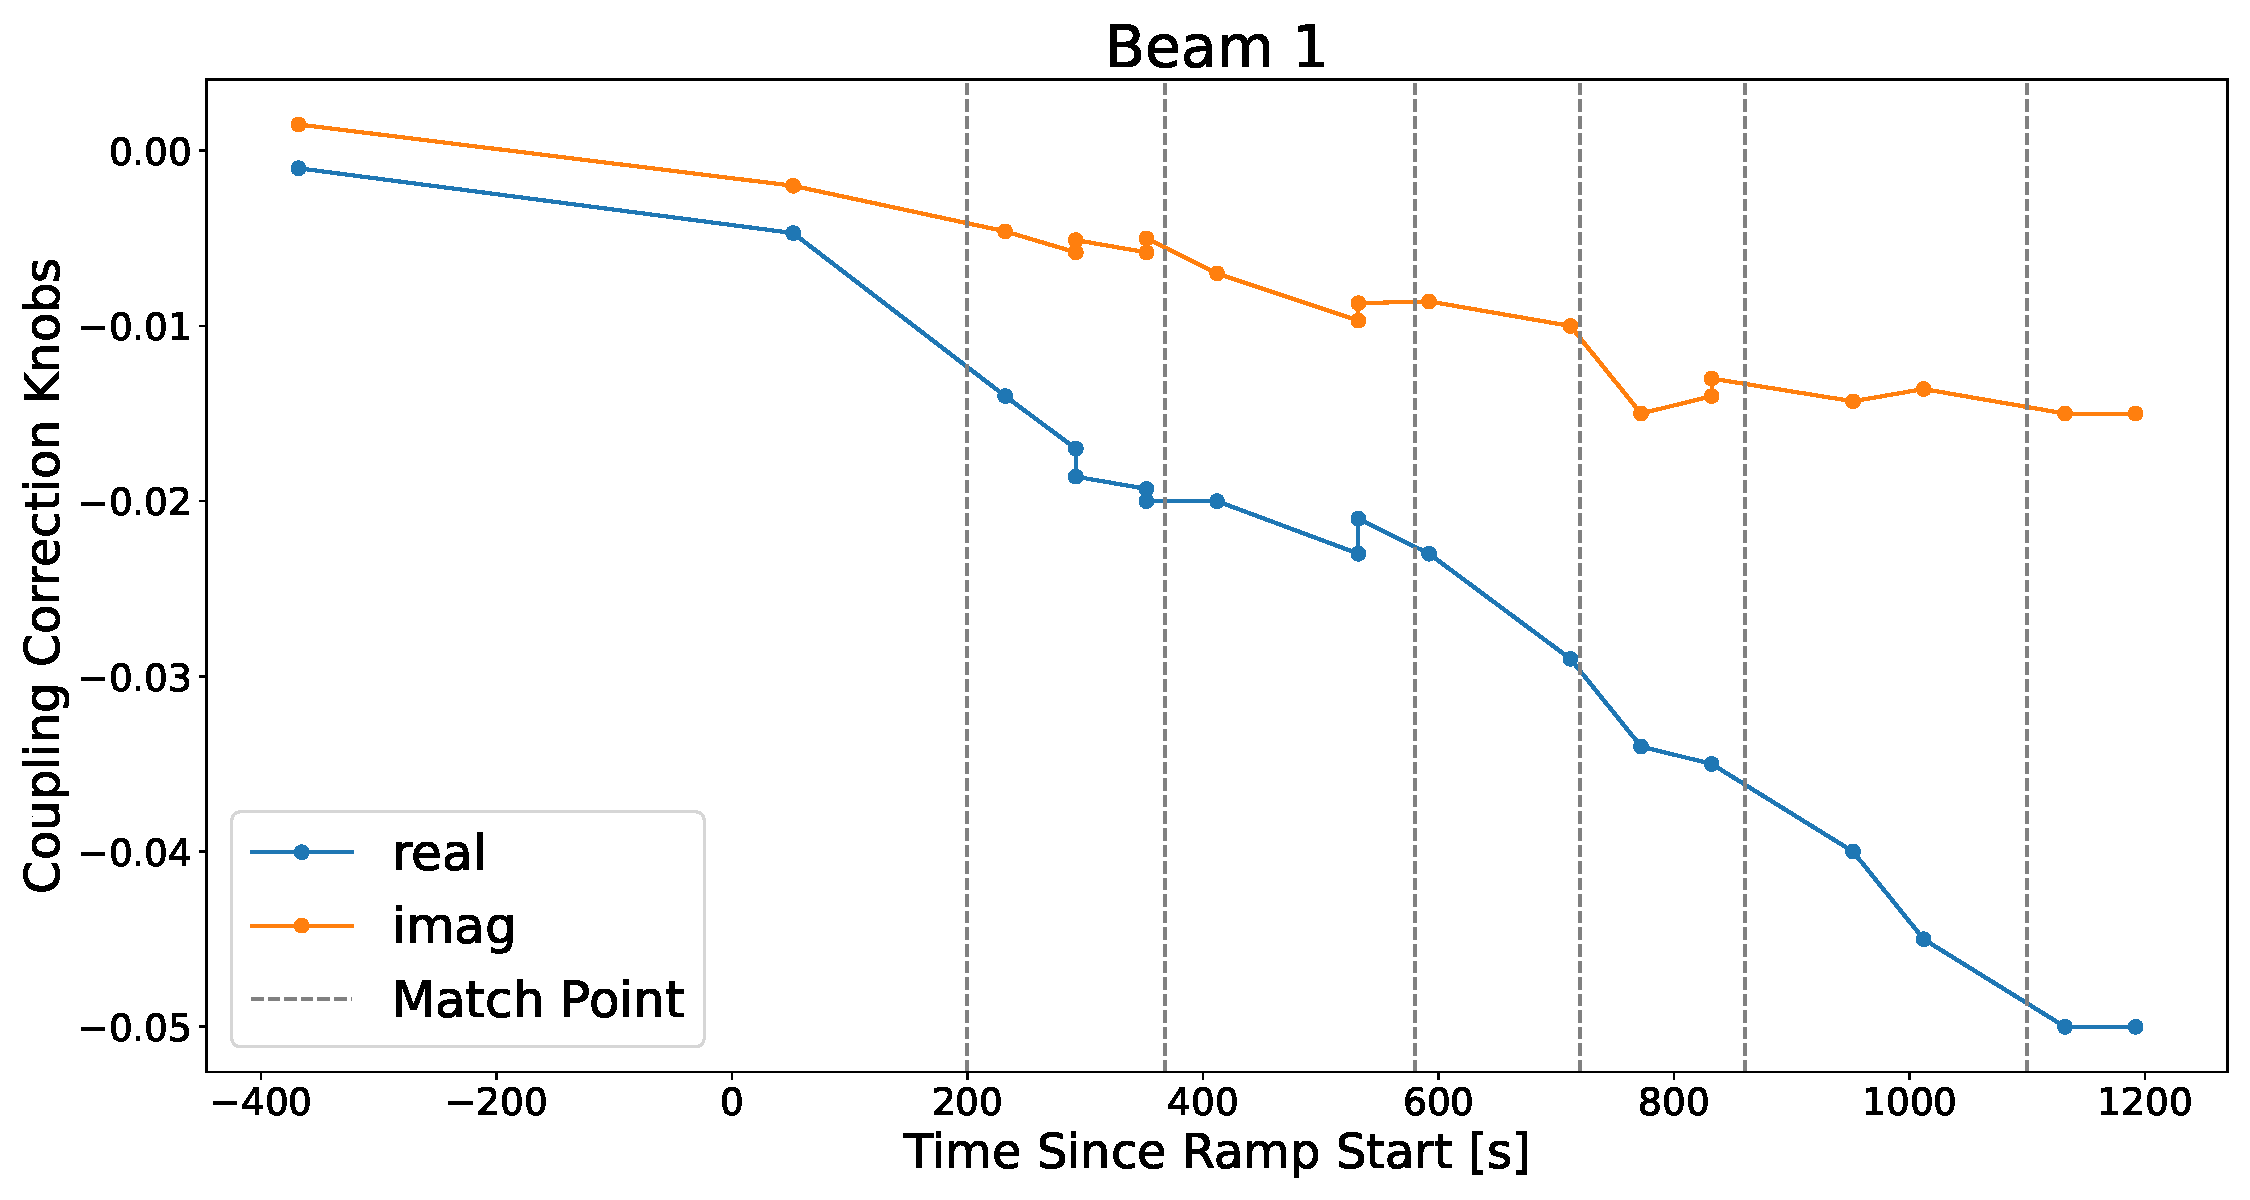
\includegraphics[width=0.49\linewidth]{images/ramp/B1_coupling_correction_knobs_in_ramp.pdf}
    \hfill
    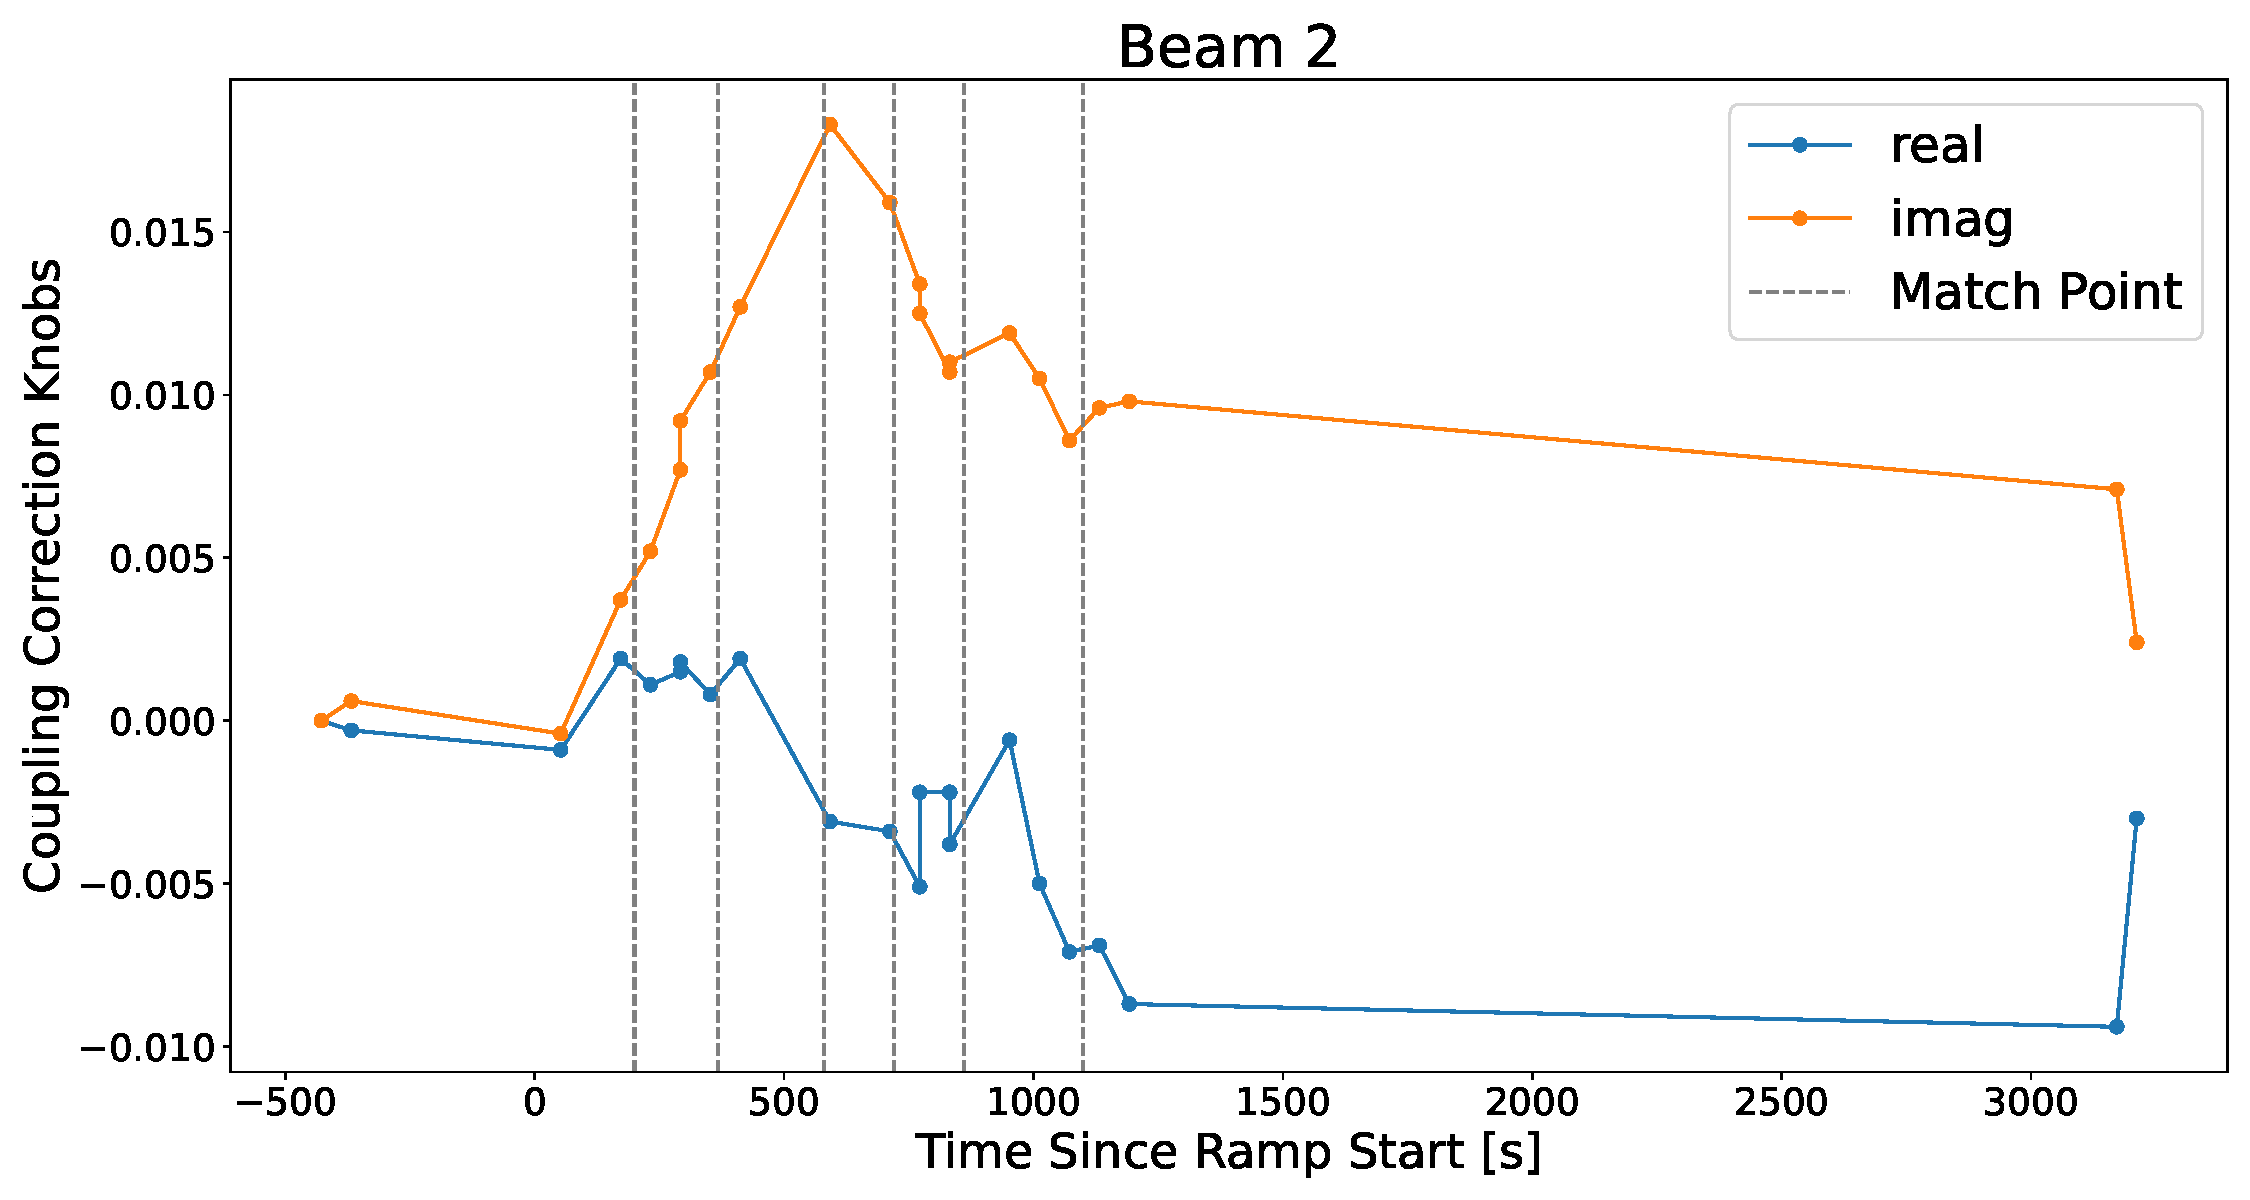
\includegraphics[width=0.49\linewidth]{images/ramp/B2_coupling_correction_knobs_in_ramp.pdf}
    
    \begin{itemize}
        \item %
            did \highl{manual coupling} measurement during the ramp because the coupling server
            \highl{failed to give} good results 
        \item %
            calculated \highl{coupling corrections} (verifying on the way that the selected model didn't deteriorate the calculations)
        \item %
            these were \highl{programmed in} to be applied during the next ramp
        \item %
            re-measure showed that we corrected \highl{$< 0.005$ at every pick-up point}
    \end{itemize}
\end{frame}


\begin{frame}{30\,cm Optics \only<2>{-- Beam~1}\only<3>{-- Beam~2}}
    \begin{center}
        \only<2>{
            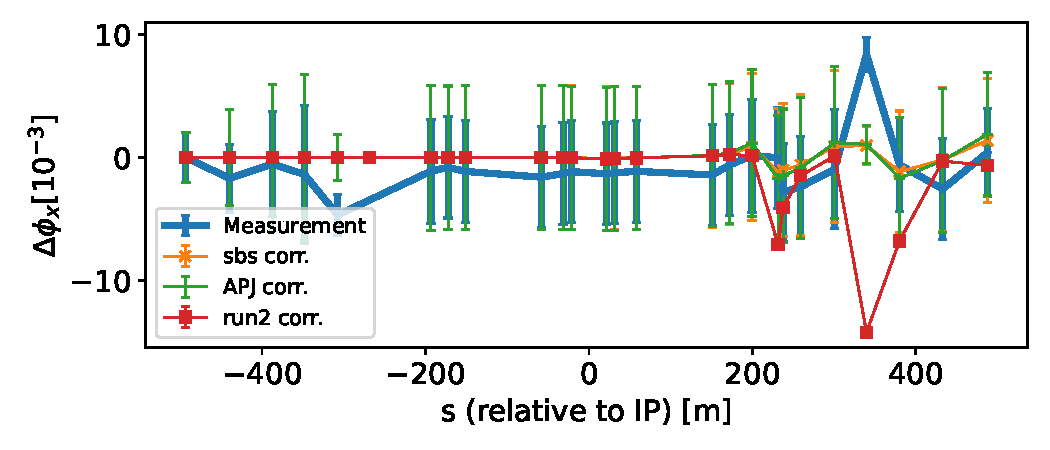
\includegraphics[width=0.4\linewidth]{images/flattop/beam1_x_IP1.pdf}
            \hspace{1cm}
            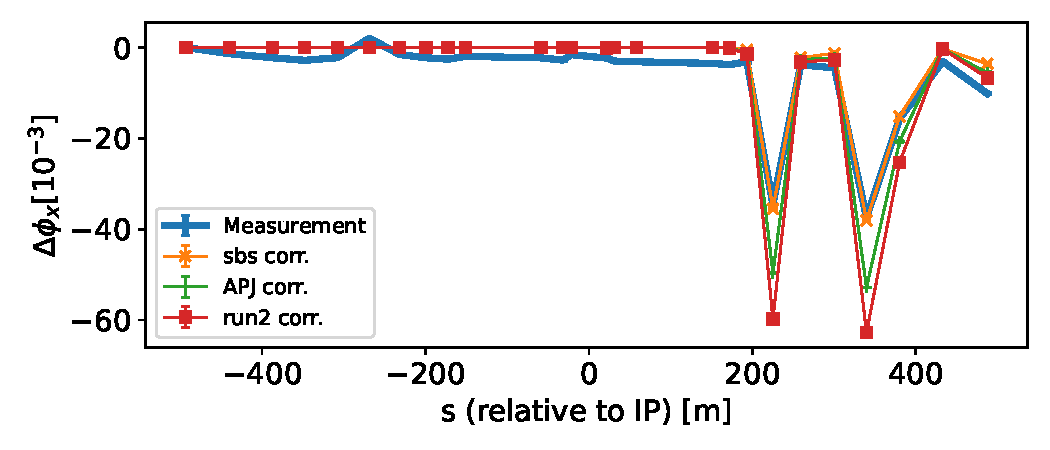
\includegraphics[width=0.4\linewidth]{images/flattop/beam1_x_IP5.pdf}
            \\
            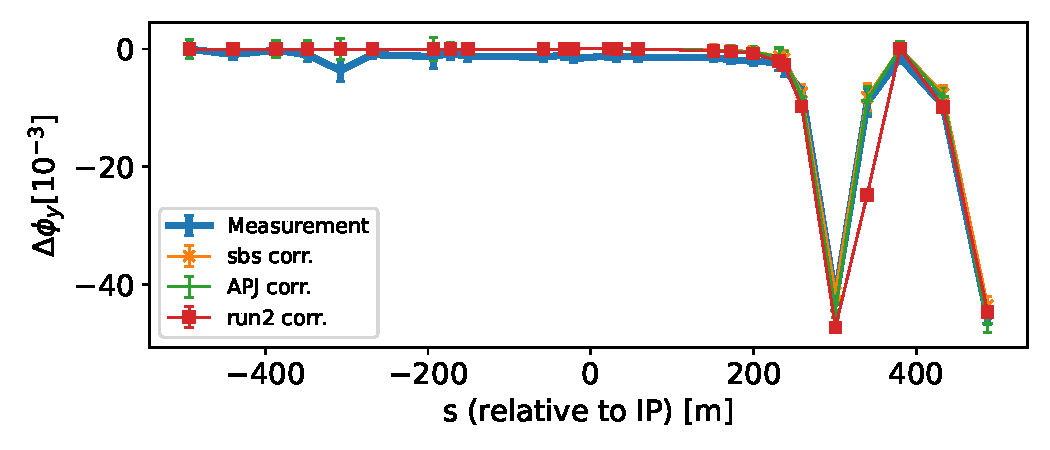
\includegraphics[width=0.4\linewidth]{images/flattop/beam1_y_IP1.pdf}
            \hspace{1cm}
            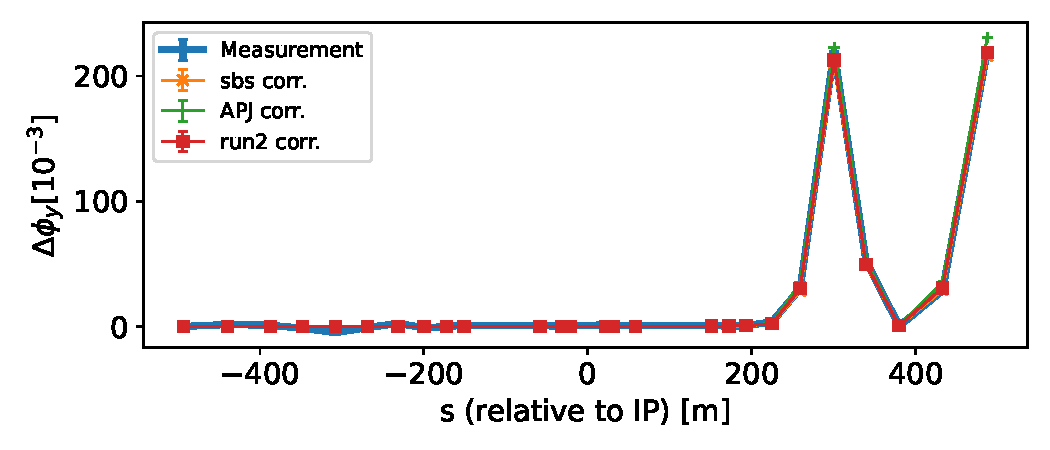
\includegraphics[width=0.4\linewidth]{images/flattop/beam1_y_IP5.pdf}
        }
        \only<3>{
            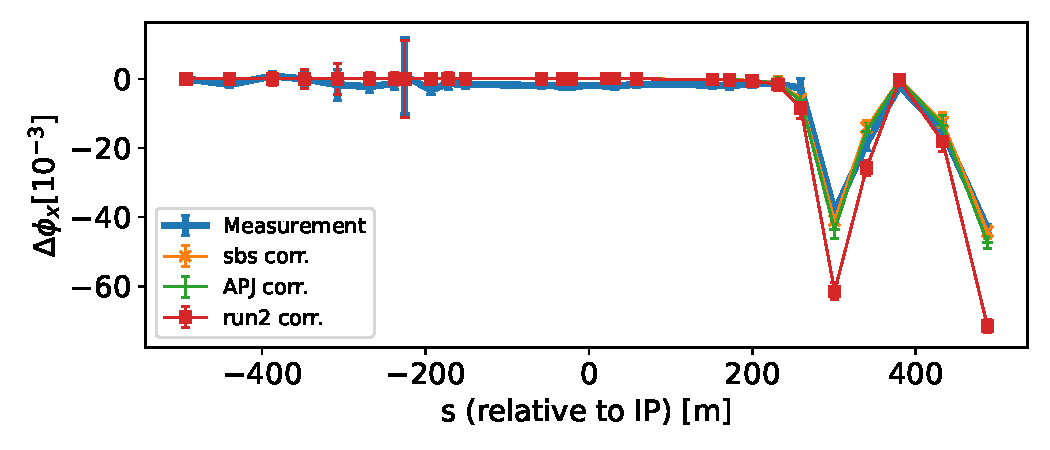
\includegraphics[width=0.4\linewidth]{images/flattop/beam2_x_IP1.pdf}
            \hspace{1cm}
            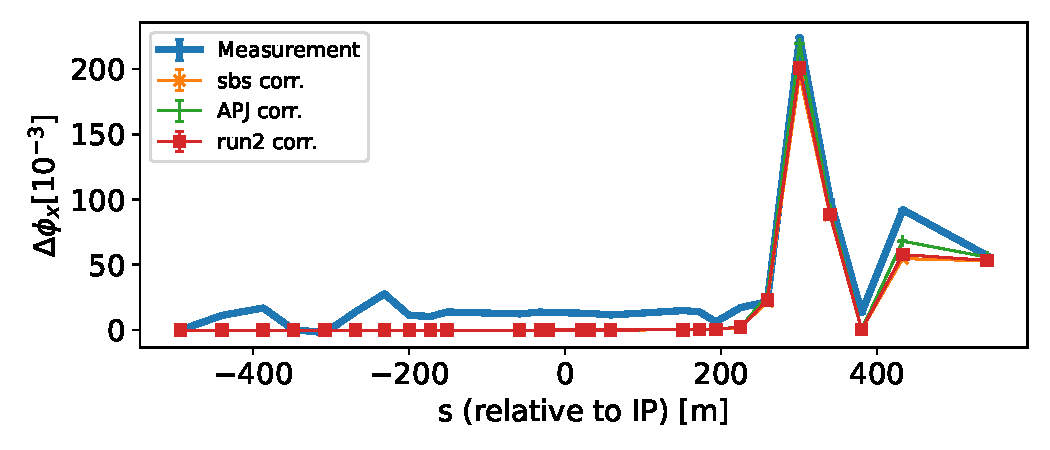
\includegraphics[width=0.4\linewidth]{images/flattop/beam2_x_IP5.pdf}
            \\
            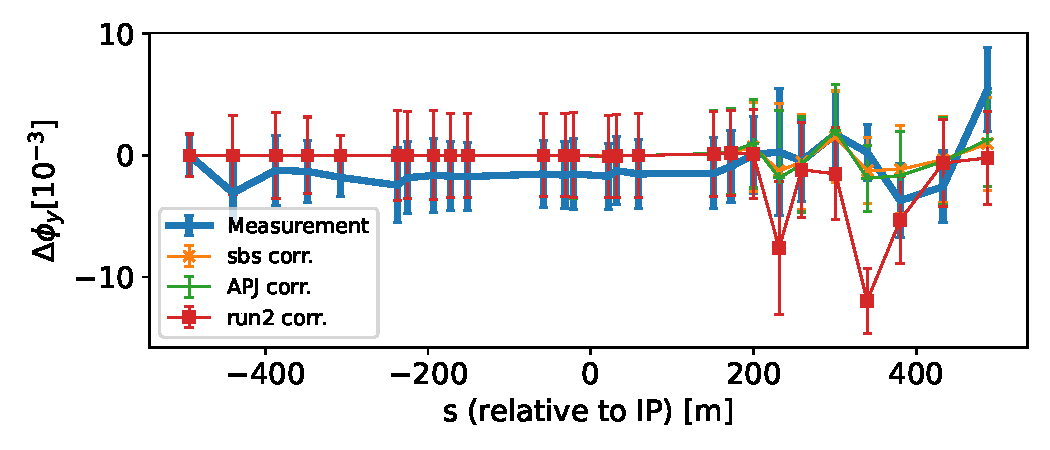
\includegraphics[width=0.4\linewidth]{images/flattop/beam2_y_IP1.pdf}
            \hspace{1cm}
            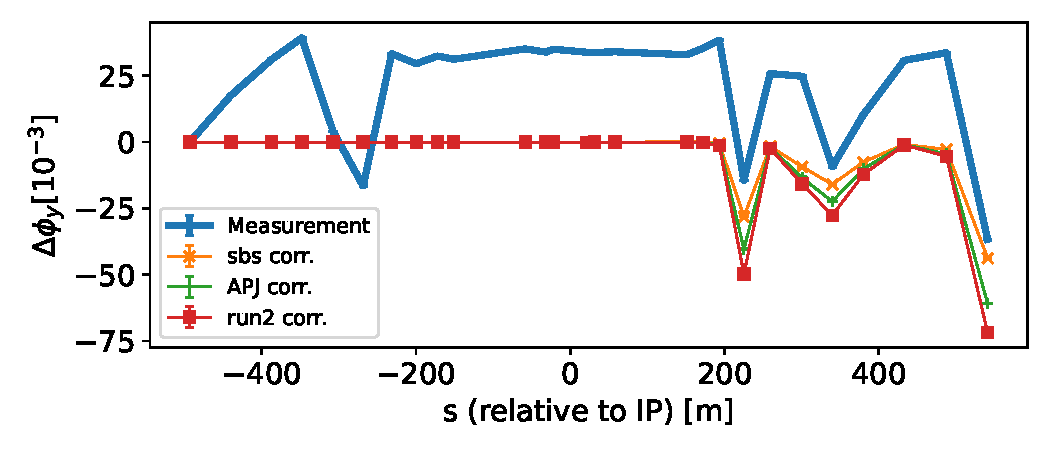
\includegraphics[width=0.4\linewidth]{images/flattop/beam2_y_IP5.pdf}
        }
        \only<1>{
        {\tiny
         \begin{tabular}{l|lSSSS|c|} \toprule
              & \textbf{Circuit}%
              & \multicolumn{4}{c|}{$\Delta k (10^{-5}\SI{}{m^{-2}})$}
              & \textbf{Polarity}%
              \\ \cmidrule{2-6}
              &
              & \multicolumn{1}{c}{\color{RunTwored}\textbf{Run 2}}
              &{\color{APJgreen}\textbf{APJ}}
              &{\color{SbSorange}\textbf{SbS}}
              &{\textbf{ML}}
              & \textbf{LSA} \\\hline \midrule
     IR1 & \texttt{ktqx1.l1} & \color{RunTwored} 1.23 & \color{APJgreen} 0    & \color{SbSorange} 1.23 &  1.23 & - \\
         & \texttt{ktqx1.r1} & \color{RunTwored}-1.23 & \color{APJgreen} 0    & \color{SbSorange}-1.23 & -1.24 & + \\
         & \texttt{ktqx2.l1} & \color{RunTwored} 0.65 & \color{APJgreen} 1.15 & \color{SbSorange} 0.41 & -0.11 & + \\
         & \texttt{ktqx2.r1} & \color{RunTwored}-1.0  & \color{APJgreen}-0.87 & \color{SbSorange}-0.70 &  0.18 & - \\
         & \texttt{ktqx3.l1} & \color{RunTwored} 1.22 & \color{APJgreen} 1.94 & \color{SbSorange} 1.22 &  0.31 & - \\
         & \texttt{ktqx3.r1} & \color{RunTwored}-1.22 & \color{APJgreen}-2.88 & \color{SbSorange}-1.22 & -0.1  & + \\\hline \midrule
     IR5 & \texttt{ktqx1.l5} & \color{RunTwored} 2.0  & \color{APJgreen} 0    & \color{SbSorange} 2.25 & \text{-} & - \\
         & \texttt{ktqx1.r5} & \color{RunTwored}-2.0  & \color{APJgreen} 0    & \color{SbSorange}-2.10 & \text{-} & + \\
         & \texttt{ktqx2.l5} & \color{RunTwored} 0.26 & \color{APJgreen} 0.38 & \color{SbSorange} 0.16 & \text{-} & + \\
         & \texttt{ktqx2.r5} & \color{RunTwored} 1.48 & \color{APJgreen} 0.93 & \color{SbSorange} 1.35 & \text{-} & - \\
         & \texttt{ktqx3.l5} & \color{RunTwored} 1.49 & \color{APJgreen} 3.40 & \color{SbSorange} 2.25 & \text{-} & - \\
         & \texttt{ktqx3.r5} & \color{RunTwored}-1.49 & \color{APJgreen}-2.46 & \color{SbSorange}-2.10 & \text{-} & + \\\hline \midrule
        \end{tabular} 
        }
        }
    \end{center}
    \begin{itemize}
        \item measurements at $\beta^*=\SI{30}{\centi\meter}$ performed
        \item corrections calculated using \highl{APJ}, \highl{SbS}, \highl{ML} and taken from \highl{run2}
        \item ML correction yield good results but are \highl{less local}
        \item APJ and SbS yield \highl{similar corrections},
            run2 corrs are over-correcting
    \end{itemize}
\end{frame}


\begin{frame}{30\,cm Optics -- before and after first global corrections}

    \begin{center}
        \begin{tikzpicture}
            \node (b1) {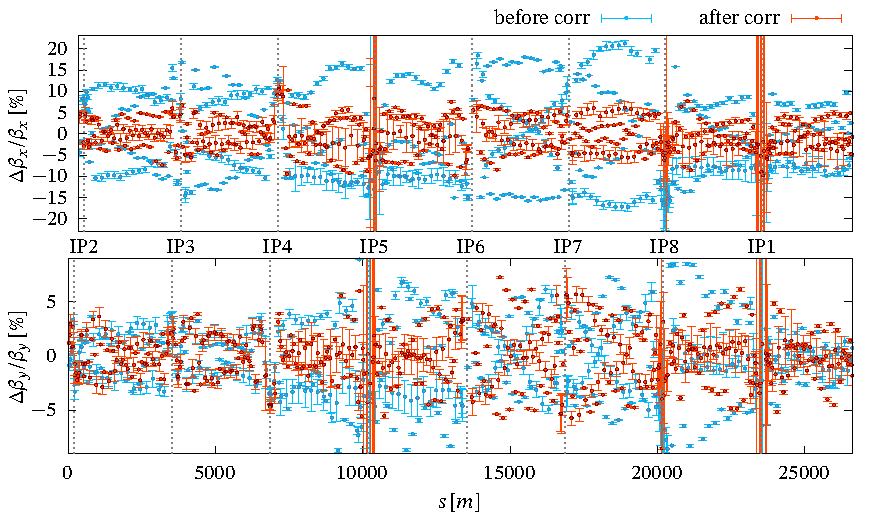
\includegraphics[width=0.5\linewidth]{images/squeeze/b1_bb_comp_after_global.pdf}};
            \node (b2) at ($(b1) + (0.5\linewidth,0)$)
            {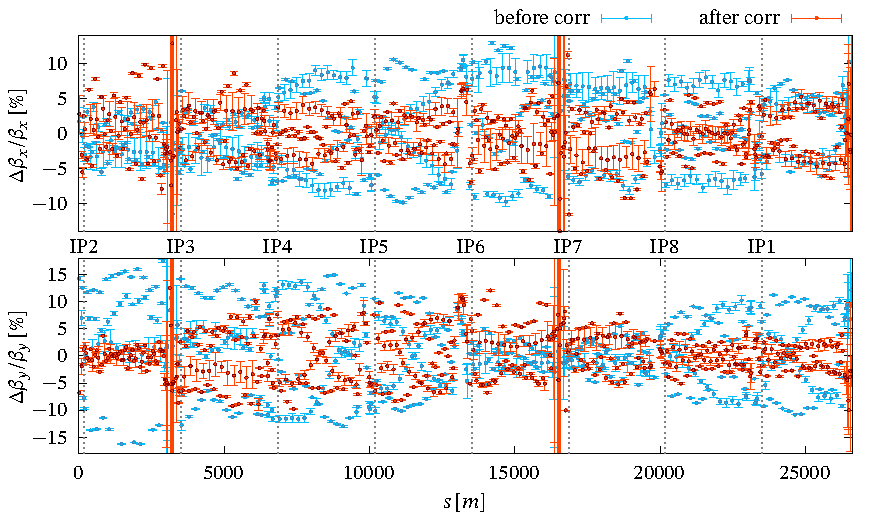
\includegraphics[width=0.5\linewidth]{images/squeeze/b2_bb_comp_after_global.pdf}};
            \bonelabel
            \btwolabel
        \end{tikzpicture}
    \end{center}
    
    \begin{itemize}
        \item after correction \highl{under 10\,\%} $\beta$~beating
    \end{itemize}
    
\end{frame}




\begin{frame}{Chromaticity}
    %\begin{center}
    %    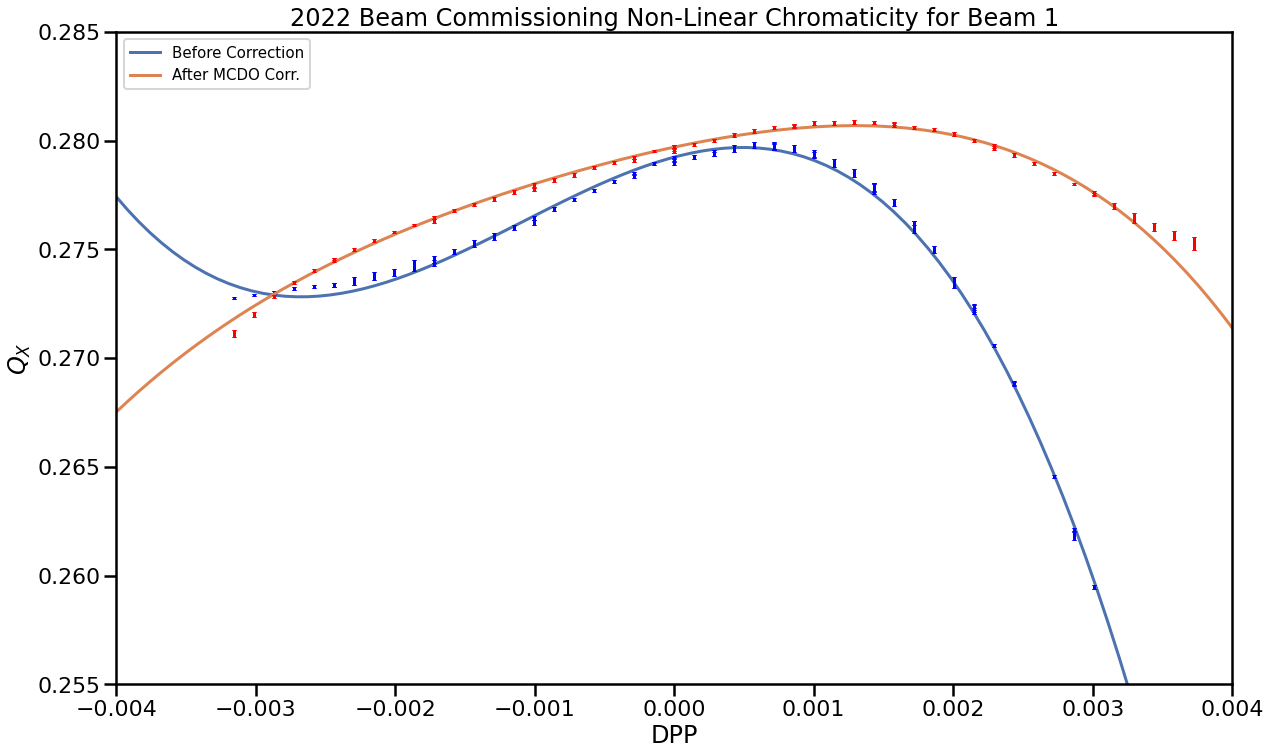
\includegraphics[width=0.49\linewidth]{images/nonlinear/comparison/qxb1q4.png}
    %\end{center}
    \begin{tabular}{l|SS|Sl}
        &\multicolumn{2}{c|}{Beam 1} & \multicolumn{2}{c}{Beam 2}  \\
        &\textbf{injection} & \textbf{60 deg} & \textbf{injection} & \textbf{60 deg} \\ 
        \hline
       $Q''_x\, [10^3]$  & -0.61 \pm 0.013 & -13.22 \pm 1.58 & -0.85 \pm 0.014 & -\\
       $Q''_y\, [10^3]$  & -0.23 \pm 0.012 &   7.83 \pm 0.08 & -0.29 \pm 0.012 & -\\
       $Q'''_x\, [10^6]$ & -1.00 \pm 0.03  & -19.56 \pm 4.73 &  0.66 \pm 0.03  & -\\
       $Q'''_y\, [10^6]$ &  0.13 \pm 0.02  &  12.35 \pm 0.37 &  0.09 \pm 0.02  & -\\
    \end{tabular}\\[1em]
    
    \begin{itemize}
        \item $Q''$ and $Q'''$ \highl{agree} with run II%, $Q'''$ does \highl{not}
        \item \highl{much larger} $dp/p$ range (2015: $\SI{2.5e-3}{}$, now: $\SI{3.5e-3}{}$)
        \item $Q''$ and $Q'''$ \highl{corrected} 
    \end{itemize}
\end{frame}



\begin{frame}{b5 Resonance}
    \begin{center}
        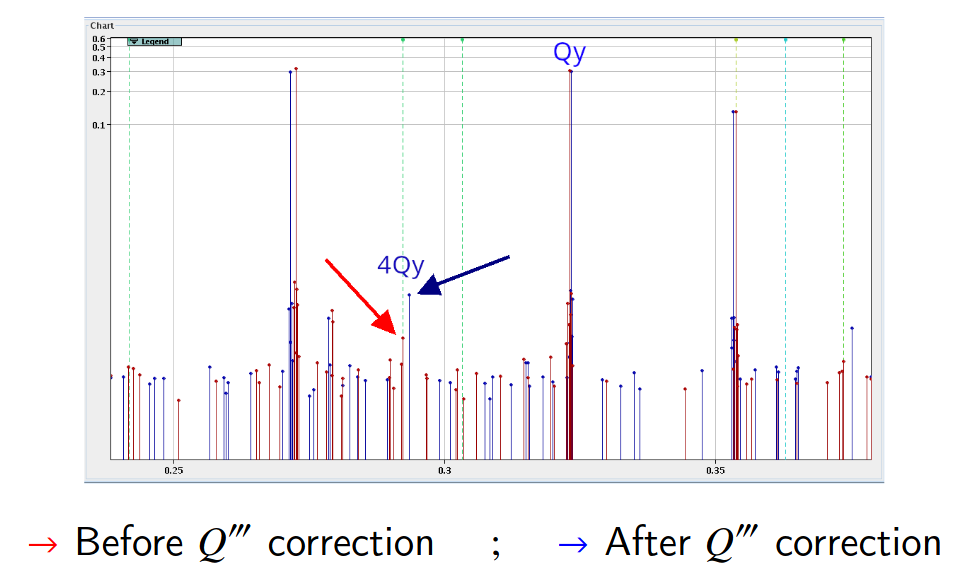
\includegraphics[width=0.5\linewidth]{images/nonlinear/b5_preliminary.png}
    \end{center}
    \begin{itemize}
        \item b5 resonance observed
        \item seems to get worse after $Q'''$ corrections
    \end{itemize}
\end{frame}



% \backcover

\end{document}
